\documentclass{article}
\usepackage{iclr2025_conference,times}
\usepackage{newtxmath}\usepackage{fontspec}\setmainfont{texgyretermes}[Extension=.otf,UprightFont=*-regular,BoldFont=*-bold,ItalicFont=*-italic,BoldItalicFont=*-bolditalic]\setmonofont{texgyrecursor}[Extension=.otf,UprightFont=*-regular,BoldFont=*-bold,ItalicFont=*-italic,BoldItalicFont=*-bolditalic]
%%%%% NEW MATH DEFINITIONS %%%%%

\usepackage{amsmath,amsfonts,bm}

% Mark sections of captions for referring to divisions of figures
\newcommand{\figleft}{{\em (Left)}}
\newcommand{\figcenter}{{\em (Center)}}
\newcommand{\figright}{{\em (Right)}}
\newcommand{\figtop}{{\em (Top)}}
\newcommand{\figbottom}{{\em (Bottom)}}
\newcommand{\captiona}{{\em (a)}}
\newcommand{\captionb}{{\em (b)}}
\newcommand{\captionc}{{\em (c)}}
\newcommand{\captiond}{{\em (d)}}

% Highlight a newly defined term
\newcommand{\newterm}[1]{{\bf #1}}


% Figure reference, lower-case.
\def\figref#1{figure~\ref{#1}}
% Figure reference, capital. For start of sentence
\def\Figref#1{Figure~\ref{#1}}
\def\twofigref#1#2{figures \ref{#1} and \ref{#2}}
\def\quadfigref#1#2#3#4{figures \ref{#1}, \ref{#2}, \ref{#3} and \ref{#4}}
% Section reference, lower-case.
\def\secref#1{section~\ref{#1}}
% Section reference, capital.
\def\Secref#1{Section~\ref{#1}}
% Reference to two sections.
\def\twosecrefs#1#2{sections \ref{#1} and \ref{#2}}
% Reference to three sections.
\def\secrefs#1#2#3{sections \ref{#1}, \ref{#2} and \ref{#3}}
% Reference to an equation, lower-case.
\def\eqref#1{equation~\ref{#1}}
% Reference to an equation, upper case
\def\Eqref#1{Equation~\ref{#1}}
% A raw reference to an equation---avoid using if possible
\def\plaineqref#1{\ref{#1}}
% Reference to a chapter, lower-case.
\def\chapref#1{chapter~\ref{#1}}
% Reference to an equation, upper case.
\def\Chapref#1{Chapter~\ref{#1}}
% Reference to a range of chapters
\def\rangechapref#1#2{chapters\ref{#1}--\ref{#2}}
% Reference to an algorithm, lower-case.
\def\algref#1{algorithm~\ref{#1}}
% Reference to an algorithm, upper case.
\def\Algref#1{Algorithm~\ref{#1}}
\def\twoalgref#1#2{algorithms \ref{#1} and \ref{#2}}
\def\Twoalgref#1#2{Algorithms \ref{#1} and \ref{#2}}
% Reference to a part, lower case
\def\partref#1{part~\ref{#1}}
% Reference to a part, upper case
\def\Partref#1{Part~\ref{#1}}
\def\twopartref#1#2{parts \ref{#1} and \ref{#2}}

\def\ceil#1{\lceil #1 \rceil}
\def\floor#1{\lfloor #1 \rfloor}
\def\1{\bm{1}}
\newcommand{\train}{\mathcal{D}}
\newcommand{\valid}{\mathcal{D_{\mathrm{valid}}}}
\newcommand{\test}{\mathcal{D_{\mathrm{test}}}}

\def\eps{{\epsilon}}


% Random variables
\def\reta{{\textnormal{$\eta$}}}
\def\ra{{\textnormal{a}}}
\def\rb{{\textnormal{b}}}
\def\rc{{\textnormal{c}}}
\def\rd{{\textnormal{d}}}
\def\re{{\textnormal{e}}}
\def\rf{{\textnormal{f}}}
\def\rg{{\textnormal{g}}}
\def\rh{{\textnormal{h}}}
\def\ri{{\textnormal{i}}}
\def\rj{{\textnormal{j}}}
\def\rk{{\textnormal{k}}}
\def\rl{{\textnormal{l}}}
% rm is already a command, just don't name any random variables m
\def\rn{{\textnormal{n}}}
\def\ro{{\textnormal{o}}}
\def\rp{{\textnormal{p}}}
\def\rq{{\textnormal{q}}}
\def\rr{{\textnormal{r}}}
\def\rs{{\textnormal{s}}}
\def\rt{{\textnormal{t}}}
\def\ru{{\textnormal{u}}}
\def\rv{{\textnormal{v}}}
\def\rw{{\textnormal{w}}}
\def\rx{{\textnormal{x}}}
\def\ry{{\textnormal{y}}}
\def\rz{{\textnormal{z}}}

% Random vectors
\def\rvepsilon{{\mathbf{\epsilon}}}
\def\rvtheta{{\mathbf{\theta}}}
\def\rva{{\mathbf{a}}}
\def\rvb{{\mathbf{b}}}
\def\rvc{{\mathbf{c}}}
\def\rvd{{\mathbf{d}}}
\def\rve{{\mathbf{e}}}
\def\rvf{{\mathbf{f}}}
\def\rvg{{\mathbf{g}}}
\def\rvh{{\mathbf{h}}}
\def\rvu{{\mathbf{i}}}
\def\rvj{{\mathbf{j}}}
\def\rvk{{\mathbf{k}}}
\def\rvl{{\mathbf{l}}}
\def\rvm{{\mathbf{m}}}
\def\rvn{{\mathbf{n}}}
\def\rvo{{\mathbf{o}}}
\def\rvp{{\mathbf{p}}}
\def\rvq{{\mathbf{q}}}
\def\rvr{{\mathbf{r}}}
\def\rvs{{\mathbf{s}}}
\def\rvt{{\mathbf{t}}}
\def\rvu{{\mathbf{u}}}
\def\rvv{{\mathbf{v}}}
\def\rvw{{\mathbf{w}}}
\def\rvx{{\mathbf{x}}}
\def\rvy{{\mathbf{y}}}
\def\rvz{{\mathbf{z}}}

% Elements of random vectors
\def\erva{{\textnormal{a}}}
\def\ervb{{\textnormal{b}}}
\def\ervc{{\textnormal{c}}}
\def\ervd{{\textnormal{d}}}
\def\erve{{\textnormal{e}}}
\def\ervf{{\textnormal{f}}}
\def\ervg{{\textnormal{g}}}
\def\ervh{{\textnormal{h}}}
\def\ervi{{\textnormal{i}}}
\def\ervj{{\textnormal{j}}}
\def\ervk{{\textnormal{k}}}
\def\ervl{{\textnormal{l}}}
\def\ervm{{\textnormal{m}}}
\def\ervn{{\textnormal{n}}}
\def\ervo{{\textnormal{o}}}
\def\ervp{{\textnormal{p}}}
\def\ervq{{\textnormal{q}}}
\def\ervr{{\textnormal{r}}}
\def\ervs{{\textnormal{s}}}
\def\ervt{{\textnormal{t}}}
\def\ervu{{\textnormal{u}}}
\def\ervv{{\textnormal{v}}}
\def\ervw{{\textnormal{w}}}
\def\ervx{{\textnormal{x}}}
\def\ervy{{\textnormal{y}}}
\def\ervz{{\textnormal{z}}}

% Random matrices
\def\rmA{{\mathbf{A}}}
\def\rmB{{\mathbf{B}}}
\def\rmC{{\mathbf{C}}}
\def\rmD{{\mathbf{D}}}
\def\rmE{{\mathbf{E}}}
\def\rmF{{\mathbf{F}}}
\def\rmG{{\mathbf{G}}}
\def\rmH{{\mathbf{H}}}
\def\rmI{{\mathbf{I}}}
\def\rmJ{{\mathbf{J}}}
\def\rmK{{\mathbf{K}}}
\def\rmL{{\mathbf{L}}}
\def\rmM{{\mathbf{M}}}
\def\rmN{{\mathbf{N}}}
\def\rmO{{\mathbf{O}}}
\def\rmP{{\mathbf{P}}}
\def\rmQ{{\mathbf{Q}}}
\def\rmR{{\mathbf{R}}}
\def\rmS{{\mathbf{S}}}
\def\rmT{{\mathbf{T}}}
\def\rmU{{\mathbf{U}}}
\def\rmV{{\mathbf{V}}}
\def\rmW{{\mathbf{W}}}
\def\rmX{{\mathbf{X}}}
\def\rmY{{\mathbf{Y}}}
\def\rmZ{{\mathbf{Z}}}

% Elements of random matrices
\def\ermA{{\textnormal{A}}}
\def\ermB{{\textnormal{B}}}
\def\ermC{{\textnormal{C}}}
\def\ermD{{\textnormal{D}}}
\def\ermE{{\textnormal{E}}}
\def\ermF{{\textnormal{F}}}
\def\ermG{{\textnormal{G}}}
\def\ermH{{\textnormal{H}}}
\def\ermI{{\textnormal{I}}}
\def\ermJ{{\textnormal{J}}}
\def\ermK{{\textnormal{K}}}
\def\ermL{{\textnormal{L}}}
\def\ermM{{\textnormal{M}}}
\def\ermN{{\textnormal{N}}}
\def\ermO{{\textnormal{O}}}
\def\ermP{{\textnormal{P}}}
\def\ermQ{{\textnormal{Q}}}
\def\ermR{{\textnormal{R}}}
\def\ermS{{\textnormal{S}}}
\def\ermT{{\textnormal{T}}}
\def\ermU{{\textnormal{U}}}
\def\ermV{{\textnormal{V}}}
\def\ermW{{\textnormal{W}}}
\def\ermX{{\textnormal{X}}}
\def\ermY{{\textnormal{Y}}}
\def\ermZ{{\textnormal{Z}}}

% Vectors
\def\vzero{{\bm{0}}}
\def\vone{{\bm{1}}}
\def\vmu{{\bm{\mu}}}
\def\vtheta{{\bm{\theta}}}
\def\va{{\bm{a}}}
\def\vb{{\bm{b}}}
\def\vc{{\bm{c}}}
\def\vd{{\bm{d}}}
\def\ve{{\bm{e}}}
\def\vf{{\bm{f}}}
\def\vg{{\bm{g}}}
\def\vh{{\bm{h}}}
\def\vi{{\bm{i}}}
\def\vj{{\bm{j}}}
\def\vk{{\bm{k}}}
\def\vl{{\bm{l}}}
\def\vm{{\bm{m}}}
\def\vn{{\bm{n}}}
\def\vo{{\bm{o}}}
\def\vp{{\bm{p}}}
\def\vq{{\bm{q}}}
\def\vr{{\bm{r}}}
\def\vs{{\bm{s}}}
\def\vt{{\bm{t}}}
\def\vu{{\bm{u}}}
\def\vv{{\bm{v}}}
\def\vw{{\bm{w}}}
\def\vx{{\bm{x}}}
\def\vy{{\bm{y}}}
\def\vz{{\bm{z}}}

% Elements of vectors
\def\evalpha{{\alpha}}
\def\evbeta{{\beta}}
\def\evepsilon{{\epsilon}}
\def\evlambda{{\lambda}}
\def\evomega{{\omega}}
\def\evmu{{\mu}}
\def\evpsi{{\psi}}
\def\evsigma{{\sigma}}
\def\evtheta{{\theta}}
\def\eva{{a}}
\def\evb{{b}}
\def\evc{{c}}
\def\evd{{d}}
\def\eve{{e}}
\def\evf{{f}}
\def\evg{{g}}
\def\evh{{h}}
\def\evi{{i}}
\def\evj{{j}}
\def\evk{{k}}
\def\evl{{l}}
\def\evm{{m}}
\def\evn{{n}}
\def\evo{{o}}
\def\evp{{p}}
\def\evq{{q}}
\def\evr{{r}}
\def\evs{{s}}
\def\evt{{t}}
\def\evu{{u}}
\def\evv{{v}}
\def\evw{{w}}
\def\evx{{x}}
\def\evy{{y}}
\def\evz{{z}}

% Matrix
\def\mA{{\bm{A}}}
\def\mB{{\bm{B}}}
\def\mC{{\bm{C}}}
\def\mD{{\bm{D}}}
\def\mE{{\bm{E}}}
\def\mF{{\bm{F}}}
\def\mG{{\bm{G}}}
\def\mH{{\bm{H}}}
\def\mI{{\bm{I}}}
\def\mJ{{\bm{J}}}
\def\mK{{\bm{K}}}
\def\mL{{\bm{L}}}
\def\mM{{\bm{M}}}
\def\mN{{\bm{N}}}
\def\mO{{\bm{O}}}
\def\mP{{\bm{P}}}
\def\mQ{{\bm{Q}}}
\def\mR{{\bm{R}}}
\def\mS{{\bm{S}}}
\def\mT{{\bm{T}}}
\def\mU{{\bm{U}}}
\def\mV{{\bm{V}}}
\def\mW{{\bm{W}}}
\def\mX{{\bm{X}}}
\def\mY{{\bm{Y}}}
\def\mZ{{\bm{Z}}}
\def\mBeta{{\bm{\beta}}}
\def\mPhi{{\bm{\Phi}}}
\def\mLambda{{\bm{\Lambda}}}
\def\mSigma{{\bm{\Sigma}}}

% Tensor
\DeclareMathAlphabet{\mathsfit}{\encodingdefault}{\sfdefault}{m}{sl}
\SetMathAlphabet{\mathsfit}{bold}{\encodingdefault}{\sfdefault}{bx}{n}
\newcommand{\tens}[1]{\bm{\mathsfit{#1}}}
\def\tA{{\tens{A}}}
\def\tB{{\tens{B}}}
\def\tC{{\tens{C}}}
\def\tD{{\tens{D}}}
\def\tE{{\tens{E}}}
\def\tF{{\tens{F}}}
\def\tG{{\tens{G}}}
\def\tH{{\tens{H}}}
\def\tI{{\tens{I}}}
\def\tJ{{\tens{J}}}
\def\tK{{\tens{K}}}
\def\tL{{\tens{L}}}
\def\tM{{\tens{M}}}
\def\tN{{\tens{N}}}
\def\tO{{\tens{O}}}
\def\tP{{\tens{P}}}
\def\tQ{{\tens{Q}}}
\def\tR{{\tens{R}}}
\def\tS{{\tens{S}}}
\def\tT{{\tens{T}}}
\def\tU{{\tens{U}}}
\def\tV{{\tens{V}}}
\def\tW{{\tens{W}}}
\def\tX{{\tens{X}}}
\def\tY{{\tens{Y}}}
\def\tZ{{\tens{Z}}}


% Graph
\def\gA{{\mathcal{A}}}
\def\gB{{\mathcal{B}}}
\def\gC{{\mathcal{C}}}
\def\gD{{\mathcal{D}}}
\def\gE{{\mathcal{E}}}
\def\gF{{\mathcal{F}}}
\def\gG{{\mathcal{G}}}
\def\gH{{\mathcal{H}}}
\def\gI{{\mathcal{I}}}
\def\gJ{{\mathcal{J}}}
\def\gK{{\mathcal{K}}}
\def\gL{{\mathcal{L}}}
\def\gM{{\mathcal{M}}}
\def\gN{{\mathcal{N}}}
\def\gO{{\mathcal{O}}}
\def\gP{{\mathcal{P}}}
\def\gQ{{\mathcal{Q}}}
\def\gR{{\mathcal{R}}}
\def\gS{{\mathcal{S}}}
\def\gT{{\mathcal{T}}}
\def\gU{{\mathcal{U}}}
\def\gV{{\mathcal{V}}}
\def\gW{{\mathcal{W}}}
\def\gX{{\mathcal{X}}}
\def\gY{{\mathcal{Y}}}
\def\gZ{{\mathcal{Z}}}

% Sets
\def\sA{{\mathbb{A}}}
\def\sB{{\mathbb{B}}}
\def\sC{{\mathbb{C}}}
\def\sD{{\mathbb{D}}}
% Don't use a set called E, because this would be the same as our symbol
% for expectation.
\def\sF{{\mathbb{F}}}
\def\sG{{\mathbb{G}}}
\def\sH{{\mathbb{H}}}
\def\sI{{\mathbb{I}}}
\def\sJ{{\mathbb{J}}}
\def\sK{{\mathbb{K}}}
\def\sL{{\mathbb{L}}}
\def\sM{{\mathbb{M}}}
\def\sN{{\mathbb{N}}}
\def\sO{{\mathbb{O}}}
\def\sP{{\mathbb{P}}}
\def\sQ{{\mathbb{Q}}}
\def\sR{{\mathbb{R}}}
\def\sS{{\mathbb{S}}}
\def\sT{{\mathbb{T}}}
\def\sU{{\mathbb{U}}}
\def\sV{{\mathbb{V}}}
\def\sW{{\mathbb{W}}}
\def\sX{{\mathbb{X}}}
\def\sY{{\mathbb{Y}}}
\def\sZ{{\mathbb{Z}}}

% Entries of a matrix
\def\emLambda{{\Lambda}}
\def\emA{{A}}
\def\emB{{B}}
\def\emC{{C}}
\def\emD{{D}}
\def\emE{{E}}
\def\emF{{F}}
\def\emG{{G}}
\def\emH{{H}}
\def\emI{{I}}
\def\emJ{{J}}
\def\emK{{K}}
\def\emL{{L}}
\def\emM{{M}}
\def\emN{{N}}
\def\emO{{O}}
\def\emP{{P}}
\def\emQ{{Q}}
\def\emR{{R}}
\def\emS{{S}}
\def\emT{{T}}
\def\emU{{U}}
\def\emV{{V}}
\def\emW{{W}}
\def\emX{{X}}
\def\emY{{Y}}
\def\emZ{{Z}}
\def\emSigma{{\Sigma}}

% entries of a tensor
% Same font as tensor, without \bm wrapper
\newcommand{\etens}[1]{\mathsfit{#1}}
\def\etLambda{{\etens{\Lambda}}}
\def\etA{{\etens{A}}}
\def\etB{{\etens{B}}}
\def\etC{{\etens{C}}}
\def\etD{{\etens{D}}}
\def\etE{{\etens{E}}}
\def\etF{{\etens{F}}}
\def\etG{{\etens{G}}}
\def\etH{{\etens{H}}}
\def\etI{{\etens{I}}}
\def\etJ{{\etens{J}}}
\def\etK{{\etens{K}}}
\def\etL{{\etens{L}}}
\def\etM{{\etens{M}}}
\def\etN{{\etens{N}}}
\def\etO{{\etens{O}}}
\def\etP{{\etens{P}}}
\def\etQ{{\etens{Q}}}
\def\etR{{\etens{R}}}
\def\etS{{\etens{S}}}
\def\etT{{\etens{T}}}
\def\etU{{\etens{U}}}
\def\etV{{\etens{V}}}
\def\etW{{\etens{W}}}
\def\etX{{\etens{X}}}
\def\etY{{\etens{Y}}}
\def\etZ{{\etens{Z}}}

% The true underlying data generating distribution
\newcommand{\pdata}{p_{\rm{data}}}
% The empirical distribution defined by the training set
\newcommand{\ptrain}{\hat{p}_{\rm{data}}}
\newcommand{\Ptrain}{\hat{P}_{\rm{data}}}
% The model distribution
\newcommand{\pmodel}{p_{\rm{model}}}
\newcommand{\Pmodel}{P_{\rm{model}}}
\newcommand{\ptildemodel}{\tilde{p}_{\rm{model}}}
% Stochastic autoencoder distributions
\newcommand{\pencode}{p_{\rm{encoder}}}
\newcommand{\pdecode}{p_{\rm{decoder}}}
\newcommand{\precons}{p_{\rm{reconstruct}}}

\newcommand{\laplace}{\mathrm{Laplace}} % Laplace distribution

\newcommand{\E}{\mathbb{E}}
\newcommand{\Ls}{\mathcal{L}}
\newcommand{\R}{\mathbb{R}}
\newcommand{\emp}{\tilde{p}}
\newcommand{\lr}{\alpha}
\newcommand{\reg}{\lambda}
\newcommand{\rect}{\mathrm{rectifier}}
\newcommand{\softmax}{\mathrm{softmax}}
\newcommand{\sigmoid}{\sigma}
\newcommand{\softplus}{\zeta}
\newcommand{\KL}{D_{\mathrm{KL}}}
\newcommand{\Var}{\mathrm{Var}}
\newcommand{\standarderror}{\mathrm{SE}}
\newcommand{\Cov}{\mathrm{Cov}}
% Wolfram Mathworld says $L^2$ is for function spaces and $\ell^2$ is for vectors
% But then they seem to use $L^2$ for vectors throughout the site, and so does
% wikipedia.
\newcommand{\normlzero}{L^0}
\newcommand{\normlone}{L^1}
\newcommand{\normltwo}{L^2}
\newcommand{\normlp}{L^p}
\newcommand{\normmax}{L^\infty}

\newcommand{\parents}{Pa} % See usage in notation.tex. Chosen to match Daphne's book.

\DeclareMathOperator*{\argmax}{arg\,max}
\DeclareMathOperator*{\argmin}{arg\,min}

\DeclareMathOperator{\sign}{sign}
\DeclareMathOperator{\Tr}{Tr}
\let\ab\allowbreak

\usepackage[hidelinks]{hyperref}
\usepackage{url,graphicx,booktabs,tabularx,xcolor,subcaption,tikz,float}
\usetikzlibrary{positioning,arrows.meta,calc}
\iclrfinalcopy

\definecolor{cV7}{HTML}{6A4CE2}\definecolor{soft}{HTML}{F3F1FB}\definecolor{line}{HTML}{8A8A8A}

\renewcommand{\topfraction}{0.9}\renewcommand{\bottomfraction}{0.7}
\renewcommand{\textfraction}{0.08}\renewcommand{\floatpagefraction}{0.85}
\setcounter{topnumber}{4}\setcounter{bottomnumber}{3}\setcounter{totalnumber}{6}
\setlength{\textfloatsep}{6pt plus 2pt minus 2pt}
\setlength{\floatsep}{5pt plus 2pt minus 2pt}
\setlength{\intextsep}{5pt plus 2pt minus 2pt}
\captionsetup{font=small,labelfont=bf,skip=2pt}
\captionsetup[sub]{font=footnotesize,skip=1pt}
\setlength{\bibsep}{1pt plus 0.5pt}

\title{Finishing Unseen DOOM Maps\\From Egocentric Sensors}
\author{Krish Jaiswal, Iyad Farooq, B Abhiruchi \& Neha Sharma \\ Team Kasukabe}

\begin{document}
\maketitle
\lhead{DevForge 2026, Track 1: Can It Play DOOM?}

\vspace{-18pt}
\begin{figure}[h]
\centering
\begin{subfigure}[t]{0.243\linewidth}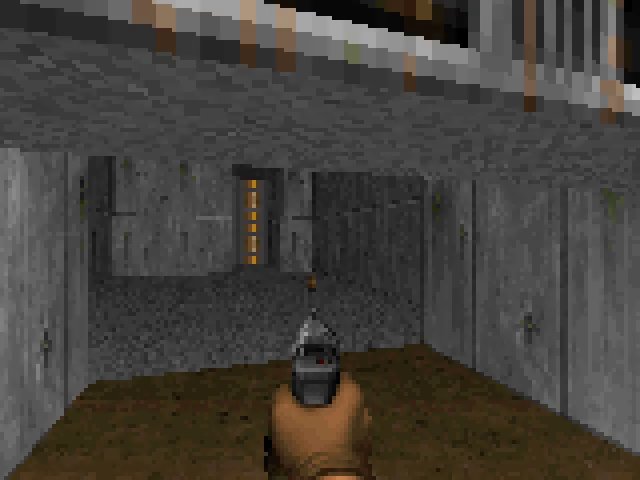
\includegraphics[width=\linewidth]{figs/f_403.png}\caption{Tier 3, exploring}\end{subfigure}\hfill
\begin{subfigure}[t]{0.243\linewidth}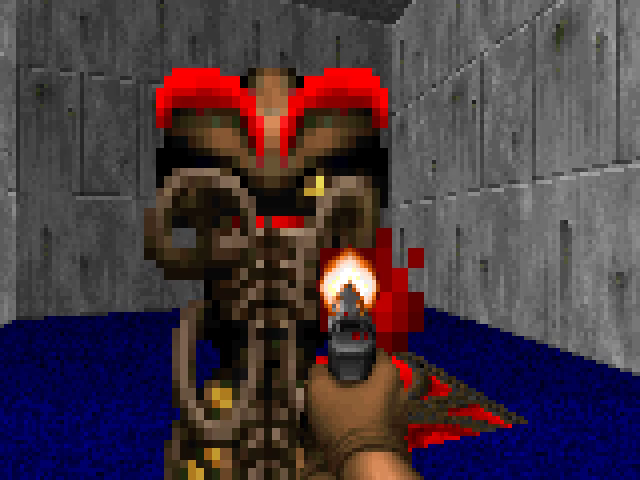
\includegraphics[width=\linewidth]{figs/f_619.png}\caption{Tier 3, fighting}\end{subfigure}\hfill
\begin{subfigure}[t]{0.243\linewidth}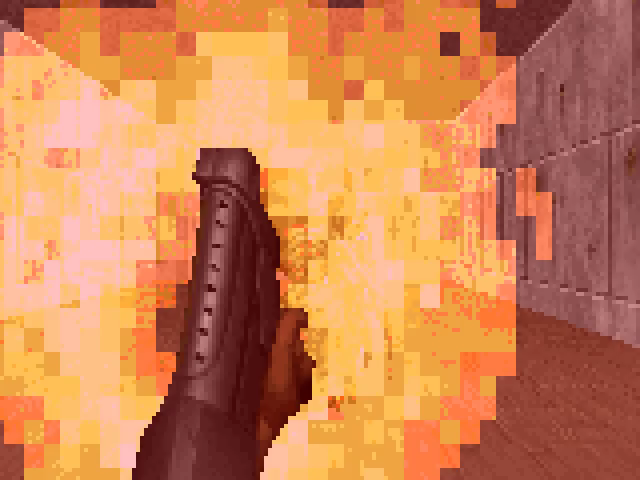
\includegraphics[width=\linewidth]{figs/f_883.png}\caption{Tier 4, firefight}\end{subfigure}\hfill
\begin{subfigure}[t]{0.243\linewidth}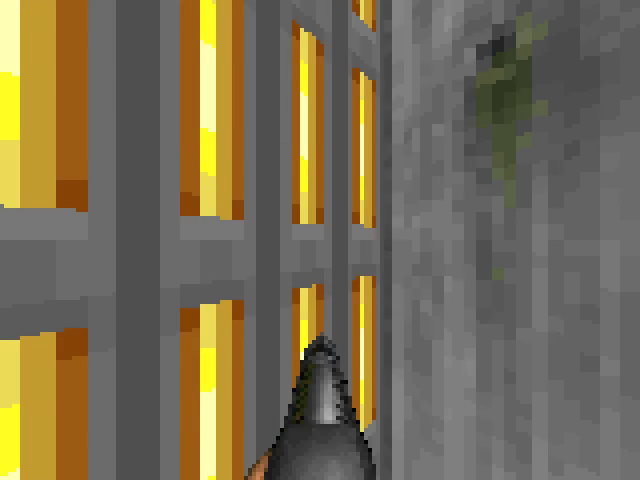
\includegraphics[width=\linewidth]{figs/f_931.png}\caption{Tier 4, near the exit}\end{subfigure}
\caption{The submitted agent on two held-out maps it never trained on, with one and two locked doors. Both episodes end at the exit.}
\label{fig:frames}
\end{figure}
\vspace{-10pt}

\section{Introduction}
The task is to play DOOM on hidden maps in four tiers (combat, doors, keycards and a gauntlet), scored on exits, doors, exploration and combat, with 40\,ms per decision on one CPU thread. Our recurrent PPO policy \citep{schulman2017ppo} trains in ViZDoom \citep{kempka2016vizdoom}, and three decisions did most of the work. We generated our own maps, because Freedoom levels are too long to finish within the 2,100 to 4,200 tick budget. We gave the reward one term per scoring category plus a potential-based guide to the next objective \citep{ng1999pbrs}. And once we saw that half of all trigger presses had no enemy in view, we penalised them. The submitted agent finishes 84\% of held-out maps and 83\% of a reserved test set run once.

\section{Method}
\begin{figure}[!b]
\centering
\resizebox{\linewidth}{!}{%
\begin{tikzpicture}[font=\footnotesize,
  enc/.style={draw=line, rounded corners=1.5pt, fill=soft, inner sep=2.2pt, align=left, text width=7.0cm, minimum height=4.6mm},
  box/.style={draw=line, rounded corners=1.5pt, fill=white, inner sep=2.5pt, align=center},
  arr/.style={-{Latex[length=1.5mm]}, draw=line, line width=0.5pt}]
\node[enc] (r) {\textbf{Rays} $64\times7$ $\rightarrow$ circular Conv1d $\times3$ $\rightarrow$ 256};
\node[enc, below=0.9mm of r] (e) {\textbf{Entities} $\le32$ $\rightarrow$ shared MLP, pooled $\rightarrow$ 128};
\node[enc, below=0.9mm of e] (v) {\textbf{Vitals} 17 + last action $\rightarrow$ MLP $\rightarrow$ 64};
\node[enc, below=0.9mm of v] (p) {\textbf{RGB-D} $4\times60\times80$ $\rightarrow$ Nature CNN (added)};
\coordinate (mid) at ($(e.south)!0.5!(v.north)$);
\node[box, minimum height=21mm, minimum width=12mm] (f) at ($(mid)+(4.55,0)$) {Concat\\448\\[2pt]FC 512\\[2pt]+ pixels};
\node[box, minimum height=21mm, minimum width=14mm, fill=cV7!12, draw=cV7, right=4mm of f] (g) {\textbf{GRU}\\\textbf{512}\\[2pt]episode\\memory};
\node[box, right=5mm of g, yshift=5mm, minimum width=27mm] (pi) {Policy: 56 combinations};
\node[box, right=5mm of g, yshift=-5mm, minimum width=27mm, dashed] (val) {Value (training only)};
\node[box, right=4mm of pi, fill=soft] (a) {Mask SELECT, $T{=}0.25$};
\foreach \n in {r,e,v,p} \draw[arr] (\n.east) -- (f.west |- \n.east);
\draw[arr] (f) -- (g); \draw[arr] (g.east) -- ++(2mm,0) |- (pi.west); \draw[arr] (g.east) -- ++(2mm,0) |- (val.west); \draw[arr] (pi) -- (a);
\end{tikzpicture}}
\caption{Policy network. All inputs come from the official observation; 2.64M parameters, 1.1\,ms median and 1.4\,ms p99 per decision on one pinned CPU core.}
\label{fig:arch}
\end{figure}


\paragraph{Network (Figure~\ref{fig:arch}).} Rays wrap around the agent, so a circular convolution treats the ray behind it as a neighbour of the ray in front. Objects come in any number and order, so a shared MLP embeds each and we pool, which keeps the encoder order-invariant \citep{zaheer2017deepsets}. With no position input, a 512-unit GRU \citep{cho2014gru} carries an episode-long state; this is how the agent returns to a locked door after finding its key. The pixel branch is the Nature CNN \citep{mnih2015dqn} behind a zero-initialised projection, so adding it did not disturb a trained policy.

\paragraph{Curriculum.} Our generator writes small UDMF maps in the four tiers using the template map's door and exit conventions, and we check each one in the real engine. We train on 240 generated maps, 41 Freedoom levels and 5 ViZDoom scenarios, select checkpoints on 24 held-out maps plus the template, and keep 24 more maps and Freedoom MAP25 to MAP32 for one final test \citep{cobbe2020procgen}.

\paragraph{Reward.} The official reward pays only for exits, deaths and kills, which is too sparse on maps that take thousands of ticks. We add a term for each scoring category, a route potential $\Phi=-d/2000$ with $d$ the remaining path through any missing keys to the exit, and from v7 a penalty for firing with no enemy within $\pm8^\circ$. The route term is a potential because shaping of the form $\Phi(s')-\Phi(s)$ leaves the optimal policy unchanged \citep{ng1999pbrs}. Appendix~\ref{app:reward} lists every weight and the reason for it.

\paragraph{Learning.} We use synchronous recurrent PPO in the style of CleanRL \citep{huang2022cleanrl} (clip 0.1, GAE $\lambda=0.95$ \citep{schulman2016gae}, $\gamma=0.99$, 128-step rollouts, 4 epochs, Adam at $2.5\times10^{-4}$), because it resumes exactly and is easy to audit, which mattered more under a deadline than raw speed. Each stage warm-starts from the previous best checkpoint. Building engines in a background thread and adding simulators took throughput from 1.3k to 6.0k transitions per second (Figure~\ref{fig:results}c).

\paragraph{Inference.} The network picks every action under two fixed settings. Masking the one combination that presses only SELECT\_NEXT\_WEAPON cut time on fists while holding bullets from 41\% to 7\%, since the engine already switches weapons on pickup and when one runs dry. Sampling at temperature 0.25 halved the back-and-forth loops of greedy play and raised our proxy from 17.08 to 17.51 on the same 300 episodes.

\section{Experiments}
\begin{figure}[!t]
\centering
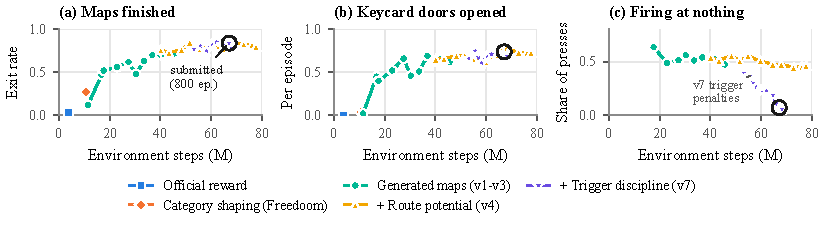
\includegraphics[width=\linewidth]{figs/fig_lineage.pdf}
\caption{Held-out results along the training lineage, 100 episodes per point. Rings mark the submitted checkpoint's 800-episode check. Panel (c) counts trigger presses with no enemy anywhere in the $90^\circ$ field of view.}
\label{fig:lineage}
\end{figure}

\begin{figure}[!t]
\centering
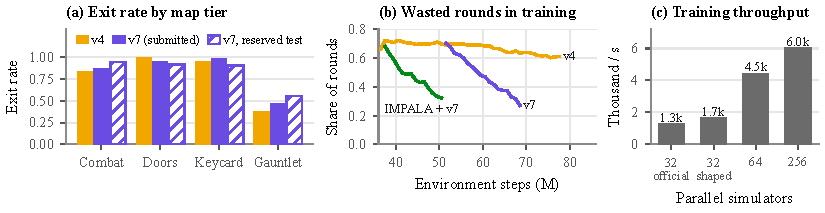
\includegraphics[width=\linewidth]{figs/fig_results.pdf}
\caption{(a) Exit rate per tier: v4 (300 episodes), submitted v7 (800), v7 on reserved test maps (288, run once). (b) Rounds fired with no enemy within $\pm8^\circ$ during training. (c) Median training throughput in thousand transitions per second.}
\label{fig:results}
\end{figure}


Checkpoints are played by the real submission agent on the 25 held-out maps with 2 seeds and both tick caps (100 episodes; finalists get 800) and ranked by a proxy of the scoring categories (Appendix~\ref{app:results}), which is our estimate and not the official score.

\paragraph{What helped.} Generated maps gave the largest jump, from 0.27 to 0.47 exits in 6M steps. The route potential took exits from 0.70 to 0.85 and improved every tier but the gauntlet, since the agent now felt its distance to the next missing key. The trigger penalties gave the cleanest gain: firing at nothing fell from 52\% to 7\% of presses and ammunition from 38.6 to 16.0 rounds per episode, while exits, locked doors and deaths all improved (Table~\ref{tab:results}).

\paragraph{What did not.} An IMPALA encoder \citep{espeholt2018impala} learned trigger discipline faster (Figure~\ref{fig:results}b) but ended level with the Nature CNN, so we kept the smaller one. Slot memory with behaviour cloning and RND \citep{burda2019rnd} matched the plain GRU at equal steps (proxy 15.3 against 14.6) at a third of its speed, so we stopped it. Full Freedoom levels stay unsolved (no exits; deaths in half the reserved episodes), as do many gauntlets (0.46 exits). Our next step is a learned egocentric occupancy map as spatial memory.

{\small
\bibliography{refs}
\bibliographystyle{iclr2025_conference}}

\appendix
\section{Training reward}\label{app:reward}
\begin{table}[H]
\centering\footnotesize
\caption{Training reward on top of the official +1 exit, $-1$ death and +0.1 kill. Each term was added in its own stage and kept only if held-out results improved. Terms may read privileged state, which the policy never sees.}
\label{tab:reward}
\setlength{\tabcolsep}{3.5pt}
\begin{tabularx}{\linewidth}{@{}l l X@{}}
\toprule
Term & Weight & Why \\
\midrule
Exit (+ health, time left) & 2 (+.25, +.25) & Largest scoring item; finishing healthy and early earns more. \\
Key / door / locked door & .5 / .1 / 1.0 & Progression is scored; locked doors gate tier 3. \\
New $128^2$ cell (once) & .025 & Exploration is scored. \\
Extra kill / damage per HP & .05 / $-$.002 & Combat is scored as kills minus damage. \\
Route potential $\Phi=-d/2000$ & $\Phi(s')-\Phi(s)$ & $d$: path left through missing keys to the exit. Keeps the optimal policy. \\
Press / round, no enemy in $\pm8^\circ$ & $-$.01 / $-$.05 & Half of all presses saw no enemy; $8^\circ\approx$ one turn step. \\
Fists with ammo / step & $-$.005 / $-$.001 & Agent drifted to fists; step cost curbs wandering. \\
\bottomrule
\end{tabularx}
\end{table}

\section{Full results}\label{app:results}

\begin{table}[H]
\centering\footnotesize
\caption{Held-out results. ``Blind'' is the share of trigger presses with no enemy anywhere in the $90^\circ$ field of view and ``Rounds'' is ammunition spent per episode. Proxy is $10\,\text{exit}(1+0.1\,\text{health}/100)+2\,\text{keys}+\text{doors}+2\,\text{locked}+0.1\,\text{cells}+0.5\,\text{kills}-0.01\,\text{damage}-\text{death}$, averaged over episodes. The 100-episode rows use greedy play. The v4 row adds the action mask, and every later row also samples at $T=0.25$. Keys, locked doors and deaths are per-episode averages.}
\label{tab:results}
\setlength{\tabcolsep}{3.1pt}
\begin{tabular}{@{}lrrrrrrr@{}}
\toprule
Checkpoint (steps; episodes) & Exit & Keys & Locked & Deaths & Blind & Rounds & Proxy \\
\midrule
Official reward only (3.7M; 100) & .03 & .26 & .00 & .11 & -- & -- & 2.37 \\
+ shaping on Freedoom (10.6M; 100) & .27 & .67 & .04 & .09 & -- & -- & 8.45 \\
+ generated maps, 256 sims (36.9M; 100) & .70 & .78 & .69 & .09 & .54 & 24.3 & 16.11 \\
+ route potential, mask (51.6M; 300) & .81 & .80 & .72 & .10 & .52 & 38.6 & 17.18 \\
\textbf{+ trigger penalties, submitted (67.2M; 800)} & \textbf{.84} & .80 & \textbf{.74} & .04 & \textbf{.07} & 16.0 & \textbf{17.60} \\
IMPALA encoder, same reward (47.9M; 800) & .83 & .81 & .72 & .03 & .14 & 15.4 & 17.31 \\
\midrule
Submitted, reserved generated maps (288) & .83 & .77 & .74 & .05 & .08 & 18.2 & 16.94 \\
Submitted, reserved Freedoom levels (96) & .00 & .00 & .00 & .54 & .00 & 10.1 & 1.54 \\
\bottomrule
\end{tabular}
\end{table}
\end{document}
